\documentclass[10pt, final]{article}

% Set up page layout
\usepackage[a4paper, margin=1in]{geometry}
% \usepackage{indentfirst}

% Language support
\usepackage{t1enc}
\usepackage[english]{babel}
\usepackage{csquotes}

% Bibliography, refs, citations
\usepackage[sorting=none, backend=biber, style=numeric]{biblatex}
\addbibresource{mmp.bib}
\usepackage{hyperref}
\hypersetup{
	colorlinks=true,
}

% Itemize with letters
\usepackage{enumitem}

% Special math representation (matrix, etc.)
\usepackage{amsmath}
\usepackage{amsfonts}

% Software code
\usepackage{listings}
\lstset{
	language=Python, 
	basicstyle={\color{blue}}
}

% Figures
\usepackage{graphicx}
\usepackage{caption}
\usepackage{subcaption}

% Graphics
\usepackage{tikz}
\usepackage{pgfplots}
\pgfplotsset{compat=1.12}
\usepackage{forest}

% Development tools - only if draft set in the documentclass options
\usepackage{ifdraft}
\ifdraft {\usepackage{showframe}}


\title{Railway Track Fault Detection\\\large Mathemathical Modeling Practice\\}
\author{Tamás DEMUS\\XP4B9D}
\date{Fall Semester 2022}

\begin{document}
	\maketitle
	\tableofcontents
	\section{Introduction}
		Analyzing images and processing the information stored within 
		is a key field of machine learning.
		Classification of different images, identifying and localizing 
		different objects are basic problems.
		Several real-life cases prove the usability of such approach 
		such as traffic sign recognition, object detection or face recognition.
		The target of current research is to endeavour to create an algorithm
		that is able to classify images taken from parts of the rail track
		to classify whether the rail is defect or not.

		A comprehensive overview about visual inspection technologies used in the railway sector is given
		in \cite{liu_review_2019}.
		It focuses on different technologies including machine learning and non machine learning applications
		and covers the overall railway sector including track, vehicle and infrastructure elements.
		The following major application categories identified: the railway track, the pantograph-catenary
		subsytem, the train body and rail infrastructure.
		The railway track is discussed in several subpoints: the detection of rail surface defects, wear and
		deformation of track components, identification of rail components and the detection and extraction  of rails.
		Current summary follows this review focusing on the track inspection methods applying machine learning
		algorithms.

		\citeauthor{xue_wang_machine-vision_2008} presents a rail surface defect detection method \cite{xue_wang_machine-vision_2008}
		based on a liner CCD followed by image processing and applying a QNN network.
		The accuracy results were evaluated and compared between QNN, ANN and SVM.
		First it detects region of interests (ROI) in the captured images by selecting pixels where the gray-level
		quantity is above a certain threshold.
		Then it searches for edges to identify the pixels that belong to certain edges.
		Then comparing this two set of points, a region of interest is defined by the presence of a set of pixels
		in both sets.
		Once this are marked, a rectangle can be drawn to enclose the region.
		Next step if to extract the features from the single ROIs.
		The features are defined based on the geometry of the flaw inside the ROI, the grey-level of the flaw pixels,
		and a so-called tansform-space, where a discrete cosine transform filter is applied.
		The obtained recalls are ranging between 86.7\% and 100\% depending on the type of flaw.

		Deep convolutional neural network (DCNN) was proposed in \cite{faghih-roohi_deep_2016} to detect surface defects of rails.
		Video recordings of rail tracks are processed by DCNNs with different sizes related to the size and number
		of the filters, number of convolutional layers and the size of the fully connected layers.
		Hyperbolic tangent and ReLU activation functions used.
		The applied dataset consits of more than 22.000 manually labelled images of 6 classes 
		(normal surface, weld, light, moderate or severe squat and joint defects).
		Input image size is 100x50 pixels and converted to grayscale.
		The multi class accuracy is ranging between 91.17\% and 92.47\%.
		The performance increases by increasing the size of the DCNN and by applying ReLU activation functions.

		Another solution for rail surface defect detection is described in \cite{ma_texture_2016}.
		Images taken by maintenance vehicles from the top and evaluated for surface defects via two SVM classifiers
		applied one after the another.
		Overall 8 defect categories differentiated including the non-defect case.
		939 manually annotated images was used for the experiments.
		A Random Forest based edge detection is followed by a Generalized Hough transform to detect the position of the rails.
		This overperformed the Canny edge detection method.
		Defect severity level classification was traced back to a texture classification task for that a Bag of Words model
		is used.
		A set of filters are used to create the feature vectors for each pixel in each image.
		From this the dictionary is created via a k-means clustering resulting in a histogram of k bins containing the number
		of pixels in each bin.
		These descriptors were fed for a $\chi^2$-kernel SVM for training.
		Besdies the dictionary texton forests were built.
		Instead of predicting the class, texton forests predict the image descriptors.
		The two methods were combined to an ensemble method by applying stacking.
		Overall 5 texton forest SVM classifier and 4 texton dictionary SVM classifier provides 9 probability vector with
		8 elements for the 8 classes.
		A second level linear-kernel SVM was fitted to these outputs.
		An accuracy of 82\% is achieved in the end.

		\citeauthor{santur_new_2017} presents a laser based imaging technology combined with deep learning model \cite{santur_new_2017}.
		The rail profile is aquired via laser scanning and afterwards a convolutional neural network is applied.
		The article distinguishes between 4 defects: cracks, abrasion, corrugation and headchecks, however only binary classification
		is implemented (faulty or not faulty image).
		The rail imaging is done via stereovision, time of flight and laser triangulation to obtain a 3d image.
		The mentioned system achieved 98\% accuracy.

		\citeauthor{li_cyber-enabled_2018} introduces a corrugation identification system that consists of an image
		acquisition system and the corresponding machine learning algorithm \cite{li_cyber-enabled_2018}.
		The images are taken from the top by equipment fitted to the underframe of the vehicle.
		The image processing covers the localization of the rail, feature extraction and corrugation recognition steps.
		Rail localization is done on the observation that the rail brightness is high and even and mostly located on the
		center of the picture.
		Features extracted by applying Fourier transformation for each column (lengthwise part of the rail surface) to 
		determine the Fourier energy spectrum after truncation and sampling to reduce the dimensionality.
		Observation taken that the longitudinal average gray value is relatively high and distributed uniformly.
		Corrugation lines represented as periodic changes of the gray value that is a sparse energy distribution
		in the frequency domain.
		Corrugation afterwards can be detected by an SVM trained on these features.
		The proposed solution reaches 99\% accuracy.
		

		\citeauthor{li_component-based_2011} presents a methodology \cite{li_component-based_2011} 
		in his work in \citedate{li_component-based_2011}
		to detect missing rail components focusing on the tie plate and it's surrounding.
		A fixed position camera is used in the research that allows a steady assessment of the track components.
		Mostly relying on edge detection mehtods on grayscale images, 
		at first detecting the tie plate itself and then the other components can be identified 
		based on the geometrical positioning.

		In his study \citeauthor{kumar_m_survey_2018} in \citedate{kumar_m_survey_2018} compares crack detection 
		methods that are based on different measurement solutions and image processing algorithms.
		The preprocessing steps are explained in detail.
		He refers to conversion grayscale images as main apprach.
		Noise reduction and the sharpening of the picture is taken as first step.
		For further evaluation he refers to several edge detection techinques that might be applied.

		In Section \ref{sec:data_desc} the dataset is introduced without any detailed analysis
		to give a first glance where the study is started. 
		Section \ref{sec:prob_stat} the main research questions stated. 
		Following in Section \ref{sec:method} a detailed dexription of the applied methodology
		and toolkits introduced.
		Section \ref{sec:results} presents the results of the study divided according to 
		the main steps of the algorithm.
		In Section \ref{sec:discussion} the results are reflected to the research questions, 
		hopefully leading to positive outcomes.
		Finally Section \ref{sec:conclusion} concludes in the overall achievements.
	\section{Dataset description} \label{sec:data_desc}
		The dataset used for this study is taken from Kaggle webpage \cite{noauthor_kaggle_nodate}
		and can be downloaded directly from 
		\url{https://www.kaggle.com/datasets/salmaneunus/railway-track-fault-detection}
		\cite*{noauthor_railway_nodate}.
		The dataset is stored in different directories related to their purpose: Train, Validation,
		or Test dataset.
		Inside each directory the classes also splitted to separate directories: Defective or Non defective.
		The directory structure along with the number of images can be seen in Table \ref{table:dir_struct}.
		\begin{table}[!ht]
			\centering
			\begin{tabular}{l c}
				Folder & Number of images \\
				\hline
				./Train/Defective & 150 \\
				./Train/Non defective & 150 \\
				./Validation/Defective & 31 \\
				./Validation/Non defective & 31 \\
				./Test/Defective & 11 \\
				./Test/Non defective & 11 \\
				\hline
			\end{tabular}
			\caption{Dataset directory structure}
			\label{table:dir_struct}
		\end{table}
		The images are taken from different perspectives, either from the top or from the side or from 
		any other direction or angle.
		The photos show different track sections, that could be a close view on the single rail or 
		a full picture taken from the entire rail section.
		The quality of the dataset is spreading between different formats, mostly consisting of jpg files.
		The size of the images are different ranging from very low to very high resolutions.
		The dataset contains only color pictures.
		Some examples are shown in Figure \ref{fig:track_non_def} and Figure \ref{fig:track_def}.
		The total size of the dataset is 2.14 GB.
		\begin{figure}[!ht]
			\centering
			\begin{subfigure}{0.3\textwidth}
				\centering
				\includegraphics[width=\textwidth]{./data/Train/Non defective/7.jpg}
				\caption{Non defective}
			\end{subfigure}
			\begin{subfigure}{0.3\textwidth}
				\centering
				\includegraphics[width=\textwidth]{./data/Train/Non defective/32.jpg}
				\caption{Non defective}
			\end{subfigure}
			\begin{subfigure}{0.3\textwidth}
				\centering
				\includegraphics[width=\textwidth]{./data/Train/Non defective/110.jpg}
				\caption{Non defective}
			\end{subfigure}
			\caption{Example images of non defective track}
			\label{fig:track_non_def}
		\end{figure}
		\begin{figure}[!ht]
			\centering
			\begin{subfigure}{0.3\textwidth}
				\centering
				\includegraphics[width=\textwidth]{./data/Train/Defective/156.jpg}
				\caption{Defective}
			\end{subfigure}
			\begin{subfigure}{0.3\textwidth}
				\centering
				\includegraphics[width=\textwidth]{./data/Train/Defective/182.jpg}
				\caption{Defective}
			\end{subfigure}
			\begin{subfigure}{0.3\textwidth}
				\centering
				\includegraphics[width=\textwidth]{./data/Train/Defective/260.jpg}
				\caption{Defective}
			\end{subfigure}
			\caption{Example images of defective track}
			\label{fig:track_def}
		\end{figure}
	\section{Problem statement} \label{sec:prob_stat}
		The algorithm targets to identify from a picture whether it represents a defective or a non defective 
		track section.
		For this purpose image manipulation technics together with machine learning algorithms, in more detail 
		neural networks applied.
		The problem formulation defines the main questions of the research to be answered:
		\begin{enumerate}[label=Q\arabic*]
			\item \label{itm:Q1} What kind of defects are represented in the images?
			\item \label{itm:Q2} Can these defects detected by applying image manipulation 
				and machine learning approach? 
			\item \label{itm:Q3} What accuracy rate can be achieved with the algorithm?
		\end{enumerate}
	\section{Methodology} \label{sec:method}
		The research can be divided to several major steps, these are described in the subsequent sections.
		The algorithm is developed in Python programming language in a form of a Jupyter notebook.
		In current research the aim was to store the different stages of the processing in different file 
		folders to allow single analytics of each processing step. 
		In each folder the same original structure is retained.
		Therefore the following data folders are differentiated.
		\begin{enumerate}
			\item \lstinline{raw} Contains the raw dataset directly copied from Kaggle.
			\item \lstinline{data} The images after data cleaning in standard format and naming.
			\item \lstinline{augmented} Additional images as result of data augmentation.
			\item \lstinline{preprocessed} The data after image processing, preprocessed for the machine learning
				algorithm. Includes both the original and augmented dataset.
		\end{enumerate}
		\subsection{Data cleaning}
			The images should be brought to the same quality in order to efficiently process them.
			This covers the identification of corrupted files, correct the wrong file formats 
			and the resolution of all issues that prevents the processing of the data along the same pipeline.
			The result of this step should be a data structure that is easy to handle and process further.
			This includes the following information.
			\begin{enumerate}
				\item Type of image, whether it is intended for training, validation or testing.
				\item Indicator of defective or non-defective class, both as integer and as string.
				\item Path of the image directory, filename and their joints as full path.
			\end{enumerate}
		\subsection{Data exploration}
			The target of this step is to get a deep understanding of the pictures contentwise.
			The main properties, such as size, color composition, orientation, what is shown and similar need to be 
			checked with respect to characteristic differences between the distinct classes.
			The size and the mean of the color components is extracted from the images and stored in the dataframe 
			of the images.
			The distribution and correlation of the images color components considering the mean values analyzed.
			A random sample of the images is taken for visualization to study the different defects of the defective class.
			As a final step, the color components were investigated in detail considering the histogram of the component
			values taken for each pixels.
			This is investigated on the RGB color model and the images were converted to HSV model to get a more
			comprehensive view.
		% \subsection{Image processing}
		% \subsection{Data augmentation}
		% \subsection{Neural network configuration}
		% \subsection{Prediction of test data}
		% \subsection{Metrics and evaluation}
	\section{Results} \label{sec:results}
		\subsection{Data cleaning}			
			The raw data from the Kaggle webpage \cite{noauthor_railway_nodate} is copied to the folder \lstinline{raw}.
			This folder is not changed during the data processing, it is used as a starting point and to preserve the 
			original data.
			During data cleaning three different file formats detected, namely \lstinline{webp}, \lstinline{jpeg} 
			and \lstinline{jpg}.
			The filenames show a much wider spread including random names, regular photo labeling (e.g.: DCIM) and others.
			As Tensorflow is not able to work with \lstinline{webp} files and to maintain the same standard along
			the dataset, all files that are not in \lstinline{jpg} format are converted to \lstinline{jpg}.
			During this conversion all the files were renamed applying an integer counter.
			The modified dataset is then stored in the \lstinline{data} folder in the same structure as in the original data.
			
			Second step is to sum all the main information of each image in a single Python DataFrame to allow easy processing.
		\subsection{Data exploration}
			The distribution of the image sizes are shown in Figure \ref{fig:shape_dist}. 
			Please note that higher detail images can be found in the corresponding Jupyter notebook, the aim in this document
			is to explain the evaluation approach and summarize the results.
			Non defective pictures have only 2 shapes, either 3000x4000 or 4000x3000, depending whether it has
			portrait or landscape orientation.
			Defective images have wider distribution in the shapes reaching as high as 8000 pixels and as low as 148 pixels.
			The minimum image size in this case is 148x194 (height x width) and the maximum is 8000x6000.
			All images have 3 color components according to RGB color model.
			\begin{figure}[!ht]
				\centering
				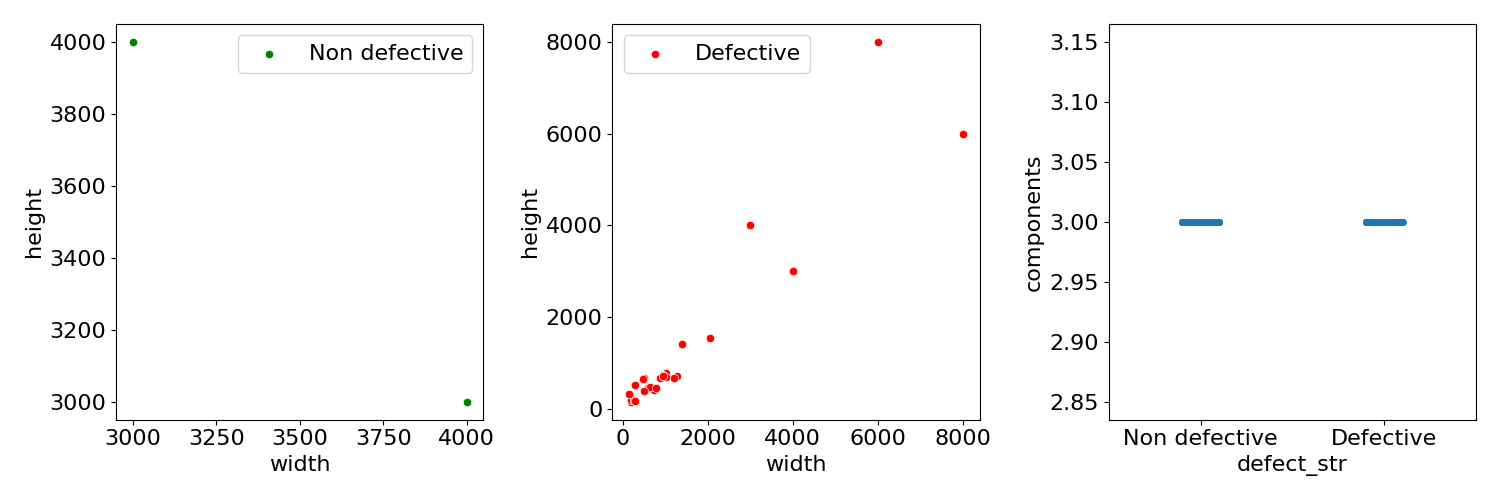
\includegraphics[width=\textwidth]{./tex_graphs/shapes.png}
				\caption{Distribution of the image shapes}
				\label{fig:shape_dist}
			\end{figure}

			The distribution and correlation of the mean of the color components with respect to the images is shown on 
			Figure \ref{fig:comp_pair}.
			\begin{figure}[!ht]
				\centering
				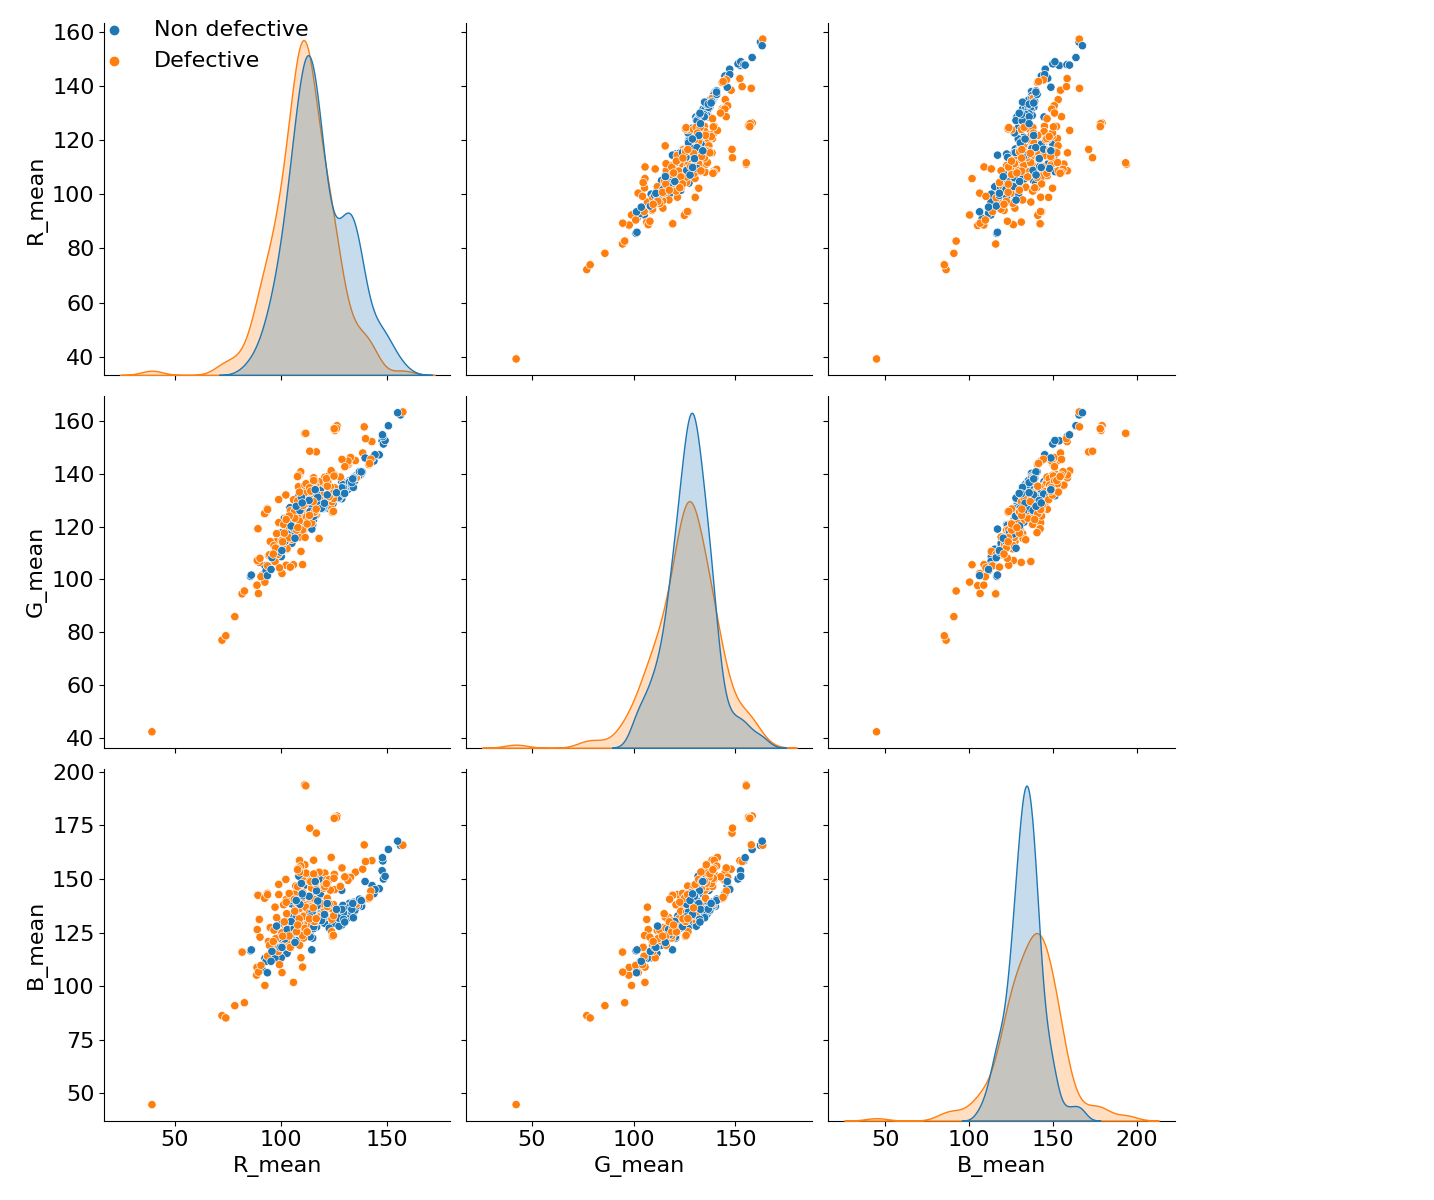
\includegraphics[width=\textwidth]{./tex_graphs/comp_pair.png}
				\caption{Color component pair analysis}
				\label{fig:comp_pair}
			\end{figure}
			The different color components show comparable histograms.
			The case of the green and blue component the non defective components show a more narrow distribution.
			The paired color components in both classes represent similar feature spaces.

			During the study of the random samples, the following defects have been identified.
			\begin{enumerate}
				\item Rail cracks. (Figure \ref{fig:def_cracked})
				\item Disjoint rail connections. (Figure \ref{fig:def_disjoint})
				\item Pitting of the rail surface. (Figure \ref{fig:def_pitting})
				\item Defect fastener. (Figure \ref{fig:def_nofix})
				\item Missing elements, e.g.: screws, springs. (Figure \ref{fig:def_missing})
			\end{enumerate}
			\begin{figure}[!ht]
				\centering
				\begin{subfigure}{0.3\textwidth}
					\centering
					\includegraphics[width=\textwidth]{./data/Train/Defective/287.jpg}
					\caption{Cracked rail}
					\label{fig:def_cracked}
				\end{subfigure}
				\begin{subfigure}{0.3\textwidth}
					\centering
					\includegraphics[width=\textwidth]{./data/Train/Defective/267.jpg}
					\caption{Disjoint rails}
					\label{fig:def_disjoint}
				\end{subfigure}
				\begin{subfigure}{0.3\textwidth}
					\centering
					\includegraphics[width=\textwidth]{./data/Train/Defective/260.jpg}
					\caption{Surface pitting}
					\label{fig:def_pitting}
				\end{subfigure}
				\begin{subfigure}{0.3\textwidth}
					\centering
					\includegraphics[width=\textwidth]{./data/Train/Defective/202.jpg}
					\caption{Fastener defect}
					\label{fig:def_nofix}
				\end{subfigure}
				\begin{subfigure}{0.3\textwidth}
					\centering
					\includegraphics[width=\textwidth]{./data/Train/Defective/215.jpg}
					\caption{Missing element}
					\label{fig:def_missing}
				\end{subfigure}
				\caption{Identified rail defects}
			\end{figure}
			The magnitude of each defect is varying in a wide range. 
			For example in case of cracked rails, from a crack of a few millimeters up to a missing rail part of several
			centimeters can be found.
			Similarly, surface pitting can range from small cracks on the surface up to severe cases, like shown in
			Figure \ref{fig:def_pitting}.

			The color component analysis on RGB and HSV colormodes revealed no exact differentiation between the classes.
			The component values highly depend on what is represented on the picture and how the photo is taken.
			For example, presence of shadow has a significant impact on the component histogram.
			An example of the analysis is shown on Figure \ref{fig:color_analysis}.
			\begin{figure}[!ht]
				\centering
				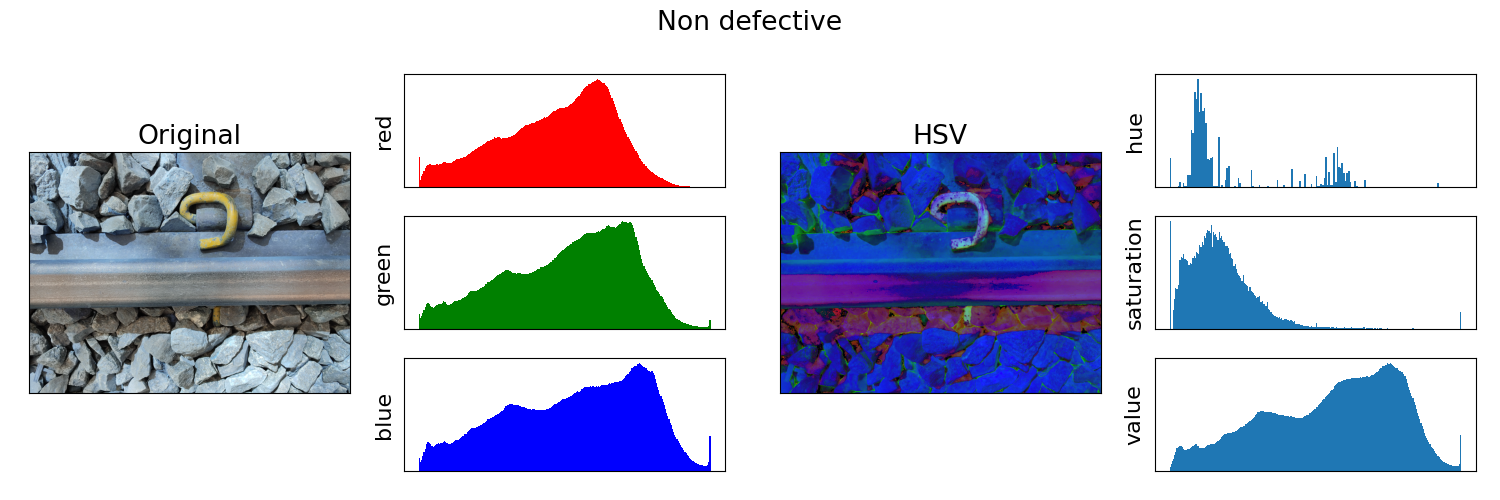
\includegraphics[width=\textwidth]{./tex_graphs/comp_analysis_1.png}
				\caption{Color component analysis on RGB and HSV color modes}
				\label{fig:color_analysis}
			\end{figure}
	\section{Discussion} \label{sec:discussion}
	\section{Conclusion} \label{sec:conclusion}
	\listoffigures
	\listoftables
	\printbibliography
\end{document}